\section{Differentialrechnung}




   

\subsubsection{Differentialquotient und Ableitung}


\begin{definition}{Sekanten-Steigung und Differentialquotient}\\
    Sei $f$ eine Funktion und $\left[x_{0}, x_{0}+h\right]$ ein Intervall im Definitionsbereich von $f$. Der Quotient
    
    $$\frac{\Delta f}{\Delta \mathrm{x}}=\frac{f\left(x_{0}+h\right)-f\left(x_{0}\right)}{h}$$
    
    heisst Differentialquotient von $f$.
\end{definition}


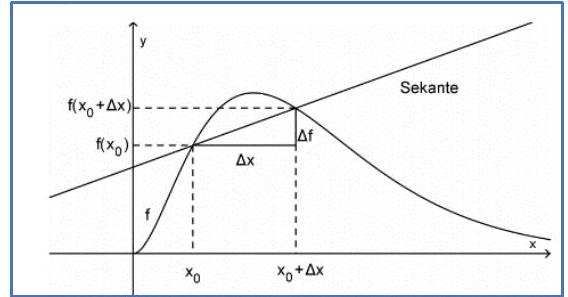
\includegraphics[scale=0.3]{2024_01_20_7bfda6c084929ccc01ffg-03.jpg}


\begin{definition}{Differenzierbarkeit}\\
    $f$ ist in $x_0$ \emph{differenzierbar}, falls der Grenzwert $\lim_{x \to x_0} \frac{f(x) -f(x_0)}{x -x_0}$
    existiert.\\
    Ist dies der Fall, wird der Grenzwert mit $f'(x)$ bezeichnet.
        $$
        f'(x_0) = \lim_{h \to 0}\frac{\Delta f}{\Delta \mathrm{x}} = \lim_{h \to 0}\frac{f(x_0 + h) -f (x_0)}{h}
        $$
    Den Grenzwert selbst bezeichnet man als Ableitung.
    \tcblower 
    \small
    Vereinfacht: Eine Funktion ist differenzierbar, falls die Kurve keine Knicke macht.
\end{definition}

\begin{formula}{Tangentengleichung}
    $
    y=f^{\prime}\left(x_{0}\right) \cdot\left(x-x_{0}\right)+f\left(x_{0}\right)
    $
\end{formula}

\begin{definition}{Stetige Differenzierbarkeit}
	Eine Funktion ist stetig differenzierbar, wenn sie differenzierbar ist und ihre Ableitungsfunktion stetig ist.
\end{definition}


\begin{definition}{n-fache Differenzierbarkeit}
	\begin{enumerate}
		\item Für $n \geq 2$ ist $f$ \emph{$n$-mal differenzierbar} in $D$ falls $f^{n-1}$ in $D$ differenzierbar ist. Dann ist $f^{(n)} \coloneqq \left(f^{(n-1)}\right)'$ und nennnt sich die $n$-te Ableitung von $f$.
		\item Die Funktion $f$ ist \emph{$n$-mal stetig differenzierbar} in $D$, falls sie $n$-mal differenzierbar ist und falls $f^{(n)}$ in $D$ stetig ist.
		\item Die Funktion $f$ ist in $D$ \emph{glatt}, falls sie $\forall n \geq 1$, $n$-mal differenzierbar ist. 
	\end{enumerate}
\end{definition}


\begin{itemize}
	\item $\exp$, $\sin$, $\cos$, $\sinh$, $\cosh$, $\tanh$ sind glatt auf $\R$
	\item Alle Polynome sind auf ganz $\R$ glatt
	\item $\ln : ]0, + \infty[ \to \R$ ist glatt
\end{itemize}

\begin{theorem}{Rechnen mit höheren Ableitungen}\\
	Sei $D \subseteq \R$, $n \geq 1$ und $f,g \to \R$ $n$-mal differenzierbar in $D$.
	\begin{enumerate}
		\item $f+g$ ist $n$-mal differenzierbar und $(f + g)^{(n)} = f^{(n)} + g^{(n)}$
		\item $f \cdot g$ ist $n$-mal differenzierbar und\\ $(f \cdot g)^{(n)} = \sum_{k=0}^n \binom{n}{k} f^{(k)} g^{(n-k)}$.
        \item $\frac{f}{g}$ ist n-mal differenzierbar falls $g(x) \neq 0, \forall x \in D$
        \item $(g \circ f)$ ist n-mal differenzierbar
	\end{enumerate}
\end{theorem}





\begin{concept}{Ableitungsregeln}
    Seien $f,g: D \to \R$  differenzierbar. Dann gelten:
    \begin{itemize}
        \item Summe/Differenz: $(f + g)'(x) = f'(x) + g'(x)$
        \item Faktor: $f(x)=a\cdot g(x) \rightarrow f'(x)=a \cdot g'(x) $
        \item Produkt: $(f \cdot g)'(x) = f'(x)g(x) + f(x)g'(x)$
        \item Quotient: $\left(\frac{f}{g}\right)'(x) = \frac{f'(x) g(x) - f(x) g'(x)}{g(x)^2}$
        \item Kettenregel: $(g \circ f)' (x) = g'(f(x)) f'(x)$
        \item Umkehrfunktion: $\left(f^{-1}\right)'(y_0) = \frac{1}{f'(x)}$
        \item Potenz/Logarithmus 1: 
        $(a^{f(x)})' = ln(a) \cdot a^{f(x)} \cdot f'(x)$

        \resizebox{\linewidth}{!}{
            $(f(x)^{g(x)})' = f(x)^{g(x)} \cdot (ln(f(x)) \cdot g(x))' =  f(x)^{g(x)} \cdot (ln(f(x)) \cdot g(x) \cdot \frac{f'(x)}{f(x)})$
            }
    \end{itemize}
    Bem. Für gerade $k$ gilt $\cosh (x)^{(k)}=\cosh (x)$ und für ungerade $k$ gilt $\cosh (x)^{(k)}=\sinh (x)$, analoges gilt für $\sinh$.
\end{concept}

 \begin{KR}{Differentialrechnung Tricks}
        \begin{itemize}
      \item Überall differenzierbar: Einheitliche Tangente (Ableitung 0 setzen) und dh: Grenzwerte müssen denselben Wert ergeben
      \item Zwei Funktionskurven berühren sich (aww): bedeutet dass sie an Stelle x0 gleichen Funktionswert und gleiche Ableitung haben
      \item Tangente bestimmen (Linearisierung): $f\left(x_{0}\right)+f^{\prime}\left(x_{0}\right)\left(x-x_{0}\right)$
    \end{itemize}
    \end{KR}

\begin{formula}{Grundfunktionen der Ableitung}
    \begin{itemize}
        \item Potenz 
    \end{itemize}
    \vspace{-3mm}
    $$f(x)=x^{n} \quad f^{\prime}(x)=n \cdot x^{n-1}$$
    \begin{itemize}
      \item Exponent
    \end{itemize}
    \vspace{-3mm}
    $$
    \begin{array}{ll}
    f(x)=a^{x} & f^{\prime}(x)=a^{x} \cdot \ln (a) \\
    f(x)=e^{x} & f^{\prime}(x)=e^{x}
    \end{array}
    $$
    
    \begin{itemize}
      \item Logarithmus
    \end{itemize}
    \vspace{-3mm}
    $$
    \begin{array}{ll}
    f(x)=\ln (x) & f^{\prime}(x)=\frac{1}{x} \\
    f(x)=\log _{a}(x) & f^{\prime}(x)=\frac{1}{\ln (a) \cdot x}
    \end{array}
    $$
\end{formula}


\begin{formula}{Ableitungen von geometrischen Funktionen}
    $$
    \arctan ^{\prime}(x) =\frac{1}{1+x^{2}}, 
    \arcsin ^{\prime}(x) =\frac{1}{\sqrt{1-x^{2}}}, 
    \arccos ^{\prime}(x) =\frac{1}{\sqrt{1+x^{2}}}
    $$

    $$
    \begin{array}{ll}
    f(x)=\tan (x) & f^{\prime}(x)=1+\tan ^{2}(x)=\frac{1}{\cos ^{2}(x)} \\
    f(x)=\cot (x) & f^{\prime}(x)=-1-\cot ^{2}(x)=-\frac{1}{\sin ^{2}(x)}
    \end{array}
    $$
\end{formula}

\begin{definition}[breakable]{Monotonie}\\
    Sei $y=f(x)$ eine differenzierbare Funktion in $D$ mit $x_{0} \in D$.
    \begin{itemize}
        \item $f'( x_{0}) = 0$ $ \Rightarrow$   $f$ konstant, bzw. horizontale Tangente
        \item $f'( x_{0}) > 0 $ $ \Rightarrow$  $f$  streng monoton wachsend.
        \item $f'( x_{0}) < 0 $ $ \Rightarrow$ $f$ streng monoton fallend.
    \end{itemize}
\end{definition}
\begin{theorem}{Krümmung}\\
    Zusammenhang zwischen 2. Ableitung und Krümmung:
    \begin{itemize}
      \item $f^{\prime \prime}\left(x_{0}\right)>0$ Konvex (Nach links/oben gekrümmt)
      \item $f^{\prime \prime}\left(x_{0}\right)<0$ Konkav (Nach rechts/unten gekrümmt)
      \item $f^{\prime \prime}\left(x_{0}\right)=0$ Keine eindeutige Krümmung
    \end{itemize}
    Bmk: Die Summe zweier konvexer Funktionen ist konvex. (konkav analog)
\end{theorem}

\begin{definition}{Wende- und Sattelpunkte}
    Als Wendepunkte werden Punkte bezeichnet bei denen sich der «Drehsinn» ändert. Wendepunkte mit horizontaler Tangente werden als Sattelpunkte oder Terrassenpunkte bezeichnet\\

Wendetangente: Tangente an einem Wendepunkt
\end{definition}



\begin{KR}{Berechnung Wendetangente}
    Ermittlung durch Lösen der Gleichung $f^{\prime \prime}(x)=0 \rightarrow x_{0}$.\\
    Bedingungen:\\
    Sei $y=f(x)$ dreimal differenzierbar

\begin{itemize}
  \item $f^{\prime \prime}\left(x_{0}\right)=0$
  \item $f^{(3)}\left(x_{0}\right) \neq 0 \quad \rightarrow$ Wendepunkt
  \item Falls zusätzlich $f^{\prime}\left(x_{0}\right)=0 \quad \rightarrow$ Sattelpunkt
\end{itemize}
    
\end{KR}

\begin{concept}{Allgemeines Kriterium}\\
    Sei $f(x)$ eine genügend oft differenzierbare Funktion

\begin{itemize}
  \item $f^{\prime}\left(x_{0}\right)=0$
\end{itemize}

Sei $n$ die Ordnung der ersten nicht verschwindenden Ableitung von $f(x)$ an der Stelle $x_{0}$:

\begin{itemize}
  \item $f^{\prime}\left(x_{0}\right)=f^{\prime \prime}\left(x_{0}\right)=\cdots=f^{(n-1)}\left(x_{0}\right)=0$
  \item $f^{(n)}\left(x_{0}\right) \neq 0$
\end{itemize}

Schlussfolgerungen:
\begin{itemize}
    \item Wenn $n$ gerade, dann gibt es ein relatives Extremum $\left(f^{(n)}\left(x_{0}\right) \neq 0\right)$
    \item Wenn $n$ ungerade, dann hat $f(x)$ an der Stelle $x_{0}$ einen Wendepunkt und damit einen Sattelpunkt
\end{itemize}
\end{concept}

\begin{KR}{Vorgehen Wende- und Sattelpunkte}
    \begin{enumerate}
  \item Erste und zweite Ableitung

  \item Wendepunkt bestimmen

\end{enumerate}

\begin{itemize}
  \item $f^{\prime \prime}\left(x_{0}\right)=0 \rightarrow x_{0}$
  \item $f^{(3)}\left(x_{0}\right) \neq 0$
\end{itemize}

\begin{enumerate}
  \setcounter{enumi}{2}
  \item Sattelpunkte bestimmen
\end{enumerate}

\begin{itemize}
  \item $f^{\prime}\left(x_{0}\right)=0$
  \item $f^{\prime \prime}\left(x_{0}\right)=0$
  \item ...
  \item $f^{(n)}\left(x_{0}\right) \neq 0$
  \item Gerade $\rightarrow$ relatives Extremum
  \item Ungerade $\rightarrow$ Sattelpunkt
\end{itemize}

\begin{enumerate}
  \setcounter{enumi}{3}
  \item $x_{0}$ in ursprüngliche Gleichung einsetzen
\end{enumerate}
\end{KR}


\begin{definition}{Relative Extrema}
    \begin{itemize}
      \item Relative Extremal-Stelle $x_0$ $\quad \Longrightarrow \quad$ Minimal-/Maximalstelle
    
      \item Relatives Extremum $y_0$ $\quad \Longrightarrow \quad$ Maximum/Minimum
    
      \item Relativer Extremal-Punkt $P_0 = (x_0, y_0)$ $\quad \Longrightarrow \quad$ Hoch-/Tiefpunkt
    
    \end{itemize}
\end{definition}

%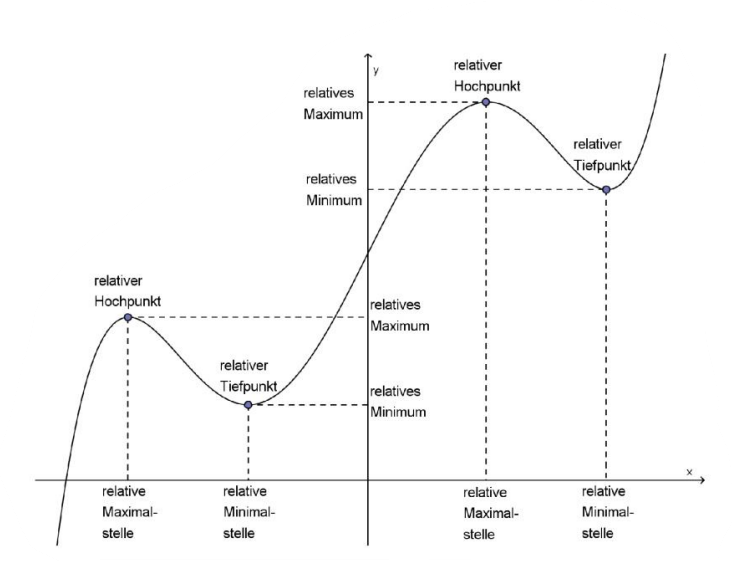
\includegraphics[scale=0.45]{Analysis1/zsf/Images/Differential/relative maxima.png}

\begin{KR}{Vorgehen relative Extrema} von $f(x) = y$:
    \begin{enumerate}
	\item Bestimme $f'(x)$ (Erste Ableitung)
	\item Bestimme NST von $f'(x)$\\
		$f'(x) = 0$ $ \Rightarrow$ $x$ lokales Extremum
	\item Bestimme $f''(x)$ (Zweite Ableitung)
		\begin{itemize}
			\item $f''(x) = 0$ $ \Rightarrow$ siehe Vorgehen Wende- und Sattelpunkte
			\item $f''(x) < 0$ $ \Rightarrow$ relatives Maximum
			\item $f''(x) > 0$ $ \Rightarrow$ relatives Minimum
		\end{itemize}
    \item In Gleichung f(x) = y einsetzen
        \begin{itemize}
            \item Hochpunkt/Tiefpunkt = $P(x, y)$
        \end{itemize}
\end{enumerate}
\end{KR}


\begin{formula}{Quadratische Funktionen}
$y=a x^{2}+b x+c$

    Nullstellen
    
    \begin{itemize}
      \item $y=a\left(x-x_{1}\right)\left(x-x_{2}\right)$
      \item $x_{0}=\frac{-b \pm \sqrt{b^{2}-4 a c}}{2 a}$
    \end{itemize}
    
    Scheitelpunkt
    
    \begin{itemize}
      \item $y=a\left(x-x_{0}\right)^{2}+y_{0}$
      \item $\mathrm{S}=\left(-\frac{b}{2 a}, \frac{4 a c-b^{2}}{4 a}\right)$
    \end{itemize}
\end{formula}































